\documentclass[headrule,footrule]{foils}

%%
%%%  Macros
%%%
%%% fonts-sil-charis for IPA in week 5

\newcommand{\logo}{HG2002 (2021)}
\usepackage[hidelinks]{hyperref}

\newcommand{\header}[3]{%
  \title{\vspace*{-2ex} \large 
    HG2002 Semantics and Pragmatics
% \thanks{Creative
%       Commons Attribution License: 
%       you are free to share and adapt as long as you give 
%       appropriate credit and add no additional restrictions: 
%       \protect\url{https://creativecommons.org/licenses/by/4.0/}.
%     }
    \\[2ex] \Large  \emp{#2} \\ \emp{#3}}
  \author{\blu{Francis Bond}   \\ 
    \normalsize  \textbf{Division of Linguistics and Multilingual Studies}\\
    \normalsize  \url{http://www3.ntu.edu.sg/home/fcbond/}\\
    \normalsize  \texttt{bond@ieee.org}}
  \MyLogo{\logo}
  % \MyLogo{奈良女子大学:欧米言語情報理論II}
  \date{#1
    \\  \url{https://bond-lab.github.io/Semantics-and-Pragmatics/}
\\[.5ex] \footnotesize Creative  Commons Attribution License:  you are free to share and adapt 
\\[-.25ex] \footnotesize   as long as you give    appropriate credit and add no
additional restrictions: 
\\ \small  \protect\url{https://creativecommons.org/licenses/by/4.0/}.
}
  % \renewcommand{\logo}{#2}
  % \special{! /pdfmark where
  %   {pop} {userdict /pdfmark /cleartomark load put} ifelse
  %   [ /Author (Francis Bond)
  %   /Title (#1: #2)
  %   /Subject (HG2002: Semantics and Pragmatics)
  %   /Keywords (Semantics, Pragmatics, Meaning)
  %   /DOCINFO pdfmark}
  %   }
  \hypersetup{%
    final       = true,
    colorlinks  = true,
    urlcolor    = blue,
    citecolor   = blue,
    linkcolor   = MidnightBlue,
    unicode     = true,
    pdfauthor   = {Francis Bond},
    pdfkeywords = {Semantics, Pragmatics, Meaning},
    pdftitle    = {#1: #2},
    pdfsubject  = {HG2002 Semantics and Pragmatics; License CC BY 4.0}
  }
}


\usepackage[a4paper,landscape]{geometry}
%\usepackage[dvips]{xcolor}
\usepackage[dvipsnames,x11names]{xcolor}
\usepackage{graphicx}
\newcommand{\blu}[1]{\textcolor{blue}{#1}}
\newcommand{\grn}[1]{\textcolor{green}{#1}}
\newcommand{\hide}[1]{\textcolor{white}{#1}}
\newcommand{\emp}[1]{\textcolor{red}{#1}}
\newcommand{\txx}[1]{\textbf{\textcolor{blue}{#1}}}
\newcommand{\lex}[1]{\textbf{\mtcitestyle{#1}}}


\usepackage{amsmath,latexsym}
\usepackage{pifont}
\renewcommand{\labelitemi}{\textcolor{violet}{\ding{227}}}
\renewcommand{\labelitemii}{\textcolor{purple}{\ding{226}}}

\newcommand{\subhead}[1]{\noindent\textbf{#1}\\[5mm]}

\newcommand{\Bad}{\emp{\raisebox{0.15ex}{\ensuremath{\mathbf{\otimes}}}}}
\newcommand{\bad}{*}

\newcommand{\com}[1]{\hfill \textnormal{(\emp{#1})}}%
\newcommand{\cxm}[1]{\hfill \textnormal{(\txx{#1})}}%
\newcommand{\cmm}[1]{\hfill \textnormal{(#1)}}%

\usepackage{relsize,xspace}
\newcommand{\into}{\ensuremath{\rightarrow}\xspace}
\newcommand{\ent}{\ensuremath{\Rightarrow}\xspace}
\newcommand{\nent}{\ensuremath{\not\Rightarrow}\xspace}
\newcommand{\tot}{\ensuremath{\leftrightarrow}\xspace}
\usepackage{url}
\newcommand{\lurl}[1]{\MyLogo{\url{#1}}}

\usepackage{mygb4e}
\let\eachwordone=\itshape
\newcommand{\lx}[1]{\textbf{\textit{#1}}}
\newcommand{\ix}{\ex\it}

\newcommand{\cen}[2]{\multicolumn{#1}{c}{#2}}
%\usepackage{times}
%\usepackage{nttfoilhead}
\newcommand{\myslide}[1]{\foilhead[-25mm]{\raisebox{12mm}[0mm]{\emp{#1}}}\MyLogo{\logo}}
\newcommand{\myslider}[1]{\rotatefoilhead[-25mm]{\raisebox{12mm}[0mm]{\emp{#1}}}}
%\newcommand{\myslider}[1]{\rotatefoilhead{\raisebox{-8mm}{\emp{#1}}}}

\newcommand{\section}[1]{\myslide{}{\begin{center}\Huge \emp{#1}\end{center}}}



\usepackage[lyons,j,e,k]{mtg2e}
\renewcommand{\mtcitestyle}[1]{\textcolor{teal}{\textsl{#1}}}
%\renewcommand{\mtcitestyle}[1]{\textsl{#1}}
\newcommand{\ja}[1]{\mtcitestyle{\makexeCJKactive #1\makexeCJKinactive}}
\newcommand{\chn}{\mtciteform}
\newcommand{\zsm}{\mtciteform}
%\newcommand{\cmn}[1]{make\cjkactive\mtciteform#1\makecjkinactive}
\newcommand{\iz}[1]{\textup{\texttt{\textcolor{blue}{\textbf{#1}}}}}
\newcommand{\con}[1]{\textsc{#1}}
\newcommand{\gm}{\textsc}
\newcommand{\cmp}[1]{{[\textsc{#1}]}}
\newcommand{\sr}[1]{\ensuremath{\langle}#1\ensuremath{\rangle}}
\usepackage[normalem]{ulem}
\newcommand{\ul}{\uline}
\newcommand{\ull}{\uuline}
\newcommand{\wl}{\uwave}
\newcommand{\vs}{\ensuremath{\Leftrightarrow}~}
%%% theta role
\newcommand{\tr}[1]{\textcolor{Chartreuse4}{\textsc{#1}}}
%%% theta grid
\newcommand{\grid}[1]{\ensuremath{\langle}\tr{#1}{\ensuremath{\rangle}}}

%%%
%%% Bibliography
%%%
\usepackage{natbib}
%\usepackage{url}
\usepackage{bibentry}
%\usepackage{CJKutf8}


\usepackage{fontenc}
\usepackage{polyglossia}
\setmainlanguage{english}
\setotherlanguages{tamil}
\setmainfont[Ligatures=TeX]{TeX Gyre Pagella}
\setsansfont[Ligatures=TeX]{TeX Gyre Heros}
\newfontfamily\ipafont{Charis SIL}
\newcommand\ipa[1]{\mtcitestyle{\ipafont #1}}


\usepackage{xeCJK}
\makexeCJKinactive
\newcommand{\zh}[1]{\mtcitestyle{\makexeCJKactive #1\makexeCJKinactive}}
%\newcommand{\ja}[1]{\makexeCJKactive #1\makexeCJKinactive}
\setCJKmainfont{Noto Sans CJK JP}
\setCJKsansfont{Noto Sans CJK SC}
\setCJKmonofont{Noto Sans CJK SC}

\newfontfamily\tamilfont[Script=Tamil]{Noto Sans Tamil}
\newfontfamily\tamilfontsf[Script=Tamil]{Noto Sans Tamil}
\newcommand{\tam}[1]{\texttamil{#1}}
%%% From Tim
\newcommand{\WMngram}[1][]{$n$-gram#1\xspace}
\newcommand{\infers}{$\rightarrow$\xspace}


\usepackage{rtrees,qtree}
\renewcommand{\lf}[1]{\br{#1}{}}
\usepackage{avm}
%\avmoptions{topleft,center}
\newcommand{\ft}[1]{\textsc{#1}}
\renewcommand{\val}[1]{\textit{#1}}
\newcommand{\typ}[1]{\textit{#1}}
\avmfont{\sc}
\avmvalfont{\sc}
\renewcommand{\avmtreefont}{\sc}
\avmsortfont{\it}


%%% From CSLI book
\newcommand{\mc}{\multicolumn}
\newcommand{\HD}{\textbf{H}\xspace}
\newcommand{\el}{\< \>}
\makeatother
\long\def\smalltree#1{\leavevmode{\def\\{\cr\noalign{\vskip12pt}}%
\def\mc##1##2{\multispan{##1}{\hfil##2\hfil}}%
\tabskip=1em%
\hbox{\vtop{\halign{&\hfil##\hfil\cr
#1\crcr}}}}}
\makeatletter

%\usepackage{tipa}
\usepackage{multicol}


\newcommand{\task}{\marginpar{\large ~~~\textbf{?}}}
\newcommand{\sh}[1]{\href{https://www.arthur-conan-doyle.com/index.php?title=#1}{#1}}

\usepackage{tikz}
\usepackage{tikz-qtree}
\usepackage{forest}



\begin{document}

\header{Lecture 1}{Introduction, Organization}{What does it mean to mean?}
\maketitle

%\include{schedule}


\myslide{Overview}

\begin{itemize}
\item Syllabus; Administrivia
\item What is semantics?
\item Why should we be interested in semantics?
\item What is meaning?
\item Meaning as an open ended conceptual system
\item Semantic problems and solutions?
\item Information Theory (new!)
\end{itemize}

\myslide{Self Introduction}

\begin{itemize}\addtolength{\itemsep}{-3mm}
%\item Francis Bond 
\item BA in Japanese and Mathematics 
\item BEng in Power and Control %(Electrical Systems Engineering)
  \raisebox{-2ex}[0mm][0mm]{
\includegraphics{pics/pwm.eps}}
\item PhD in English on  \textit{Determiners and Number in English
  contrasted with Japanese,  as exemplified in Machine
  Translation} 
\item 1991-2006 NTT (Nippon Telegraph and Telephone)
  \begin{itemize}
  \item Japanese - English/Malay Machine Translation
  \item Japanese corpus, grammar and ontology (Hinoki)
  \end{itemize}
\item 2006-2009 NICT (National Inst. for Info. and Comm. Technology)
  \begin{itemize}
  \item Japanese - English/Chinese Machine Translation
  \item Japanese WordNet
 
 \end{itemize}
\item 2009- NTU
\end{itemize}


\myslide{Administrivia}
\begin{description}\addtolength{\itemsep}{-5mm}
\item [Coordinator]  Francis \ul{Bond} 
{\small \url{<bond@ieee.org>} !\url{<fcbond@ntu.edu.sg>}}
% \item [Tutor]  James Sneed \ul{German}, Joanna \ul{Sio} Ut Seong 
% {\small \url{<jsgerman@ntu.edu.sg; neosome@gmail.com>}}
\item Details about the tutor, lecture and tutorial times and
  locations are online:
  \begin{center}
    \url{http://compling.hss.ntu.edu.sg/courses/hg2002/}    
  \end{center}


% \item [Tutorials] 
%   \begin{itemize}
%   \item Mon: 11:30--12:30 (T1: S3.2SR1 \textbf{FB}; T2: SPMS-TR+20 \textbf{JS})
%   \item 12:30--13:30 (T3: TR+19 \textbf{JS}); 14:30--15:30 (T3: TR+19 \textbf{JS});
%   \end{itemize}
% \item[Office hours] ~
%   \begin{tabular}[t]{llr}
% Francis & Tuesday &  14:00--15:00   \\  
% Francis & Thursday &  10:00--11:00   \\
% Joanna  & Friday & 9:30--11:30 
%   \end{tabular}
% \\[2ex] Or by appointment: email us (we can't guarantee to always be there).
\end{description}



\myslide{100\% Continuous Assessment}

% 1. Final in-class assessment   30%
% 2. Mid-term quiz  20%
% 3. Project  40%
% 4. Class participation  10%

\begin{itemize}
\item Class Participation (10\%)
\item Assignment (30\%)
  \begin{itemize}
  \item The assignment involves some annotation 
    \\ --- determining the meaning of words in context
  \end{itemize}
\item Mid-term Quiz (20\%)
\item Final Exam (40\%)
\end{itemize}
% \begin{itemize}
%   \item Give a precise and explicit model of some phenomenon not covered in class
%   \item The talk must motivate the choice of phenomenon
%   \item You need only cover  existing work
%   \item In-class presentation with slides or handouts, not to exceed 17 minutes (12 presentation, 5 QA)
%   \item You should choose something relevant to your final project if possible
%   \end{itemize}
% \newpage
% \item Individual Project (40\%) 
%   \begin{itemize}
%   \item Give a precise and explicit model for some phenomenon not covered in class
%     \begin{itemize}
%     \item You should give attested and constructed examples
%     \item You should clearly indicate what you can and can't explain
%     \item It is expected that you can not explain everything perfectly
%     \item Your model should make clear predictions
%     \end{itemize}
%   \item The paper must motivate the choice of phenomenon
%   \item You should cover relevant existing work \emp{and add something new}
%   \item LMS format, not to exceed 12 pages
%   \end{itemize}
% \end{itemize}


\myslide{Guidelines for Written Work in LMS}

\begin{itemize}
\item All assignments must follow the \textit{Guidelines to Submitting Written Work for the Division of Linguistics and Multilingual Studies}
  \begin{itemize}
  \item You can get it from:
\url{http://www.soh.ntu.edu.sg/Programmes/linguistics/studentresources/Documents/Linguistics%20Assignment%20Guidelines.pdf}
  \item I am \textbf{strict} about assignment length and format
    \\ learning to read and follow instructions is a \textbf{very} useful skill
  \item Useful advice on citation, transcription, formatting
  \item I also recommend my own \textit{(Computational) Linguistics Style Guide}:
 \url{http://www3.ntu.edu.sg/home/fcbond/data/ling-style.pdf}
  \item Proper citation is important 
    \\ --- failure to cite is plagiarism --- \textbf{fail subject}
 \\ See the NTU code of academic integrity 
 \\\url{http://www.ntu.edu.sg/ai/Pages/index.aspx}
  \end{itemize}
\end{itemize}


% \myslide{Course Content}

% This course introduces basic corpus skills for linguists:
% \begin{itemize}
% \item Marking up extra information
% \item Selecting text
% \item The range of existing corpora
% \item How to build your own corpus
% \item Using corpora to test linguistic hypotheses
% \item Using corpora to train language tools
% \end{itemize}

\myslide{What do you learn?}


Students will learn semantics at an introductory level and they will
acquire semantic analysis skills. With these skills and their
knowledge of semantic approaches, students will be able to approach
natural language data, as well as develop awareness of the inherent
connections between semantics and other branches of linguistics.


\myslide{Textbook and Readings}

\begin{itemize}
\item Textbooks
  \begin{itemize}
  \item Saeed, John (2009). \textit{Semantics}. 3rd Edition. Wiley-Blackwell. (\textbf{required})
  \item Lyons, John (1977) \textit{Semantics}.  Cambridge University Press (\textbf{recommended})
  \end{itemize}
\item From next week, I expect you to read all chapters assigned
  before class.
  \begin{itemize}
  \item And attempt the tutorial questions!
  \end{itemize}
\item Ideas from the book will be pursued in parallel with the
  topics given above.
\end{itemize}

% Other References

% Biber, D., S. Conrad \& R. Reppen, Corpus Linguistics: Investigating Language Structure and Use. Cambridge University Press, 1998.

% Kennedy, G. An Introduction to Corpus Linguistics. Longman, 1998.

% McEnery, Tony et al. Corpus-Based Language Studies: An Advanced Resource Book. Routledge, 2006.

% McEnery, Tony and Andrew Wilson Corpus Linguistics 2nd ed, Edinburgh UP, 2001

% Sinclair, John. Corpus Concordance Collocation. Oxford: Oxford UP, 1991


\myslide{Student Responsibilities}

By remaining in this class, the student agrees to:
\begin{enumerate}
\item  Make a good-faith effort to learn and enjoy the material.
\item  Read assigned texts, participate in class discussions and
  activities.
  \begin{itemize}
  \item Question marks mean I will ask you something\task
  \end{itemize}
\item Submit assignments on time.
\item Attend class at all times, barring special circumstances (see below).
\item Get help early: approach us when you first have trouble understanding a concept or homework problem rather than complaining about a lack of understanding afterward.
\item Treat other students with respect in all class-related activities, including on-line discussions.
\end{enumerate}
\myslide{Attendance}
\begin{enumerate}
\item You are expected to attend all classes.
\item Be on time - lateness is disruptive to your own and others' learning.
\item Valid reasons for missing class include the following:
\begin{enumerate}
\item A medical emergency (including mental health emergencies)
\item A family emergency (death, birth, natural disaster, etc)
\item A non-movable special event (sports competition, interview,
  nobel peace prize, \ldots{})
\end{enumerate}
You must provide documentation to the student office who then contacts
me.
\item There will be significant material covered in class that is not in your readings.  You cannot expect to do well without coming to class.
\item If you miss a class, it is your responsibility to get the notes, any handouts you missed, schedule changes, etc. from a classmate.
\end{enumerate}

\myslide{Remediation and Academic Integrity}
\begin{enumerate}
\item No late work will be accepted, except in the case of a documented excuse.
\item For planned, justified, absences on class days or days on which assignments are due, advance notice must be provided.
\item Cheating will not be tolerated. Violations, including plagiarism, will be seriously dealt with, and could result in \textbf{a failing grade for the entire course}.
\item For all other issues of academic integrity, refer to the University Honour Code 
\item As always, use your common sense and conscience.
\end{enumerate}


\myslide{The winning strategy}

\begin{itemize}
\item Read the books before class (and after again, if necessary)
\item Try to answer when there is a task\task
  \begin{itemize}
  \item there often is no one right answer, so don't be shy
  \end{itemize}
\item Work together: make study groups
\item Homework/Tutorials: Discuss as much as you want, write up your own answers
  \begin{itemize}
  \item You should read the chapter and attempt the tutorials before class
  \end{itemize}
\item Exams: No discussion
\item Ask questions \ldots\   early and often!
\end{itemize}

\myslide{The winning strategy (zoom edition)}

\begin{itemize}
\item Read the books and watch the videos before class (and after again, if necessary)
\item Answer in the chat when there is a task\task --- multiple
  answers are fine 
  \begin{itemize}
  \item there often is no one right answer, so don't be shy
  \end{itemize}
\item Work together: make study groups
\item Homework/Tutorials: Discuss as much as you want, write up your own answers
  \begin{itemize}
  \item You should read the chapter and attempt the tutorials before class
  \end{itemize}
\item Exams: No discussion
\item Ask questions \ldots\ early and often! Email \url{bond@ieee.org}
\end{itemize}

\section{Introduction to Semantics}

\myslide{What is Semantics?}
\begin{itemize}
\item Very broadly, semantics is the study of meaning
  \begin{itemize}
  \item Word meaning
  \item Sentence meaning
  \item Meaning in context
  \end{itemize}
\item Why do we want to study meaning?
\item What kind of knowledge does it take for a speaker to produce language and for a hearer to comprehend language? 
\end{itemize}

\myslide{Layers of Linguistic Analysis}
\begin{enumerate}\addtolength{\itemsep}{-0.75ex}
\item Phonetics \& Phonology
\item Morphology
\item Syntax
\item Semantics
\item Pragmatics
\end{enumerate}
Two theories
\begin{itemize}
\item Semantics is \txx{autonomous}, a separate module
\item Semantics is \txx{integrated} with other knowledge, inseparable
  \begin{itemize}
  \item linguistic knowledge is inseparable from encyclopedic knowledge
  \end{itemize}
\end{itemize}

\myslide{Do we share a common conceptual system?}

\begin{itemize}
\item What is a \lex{high school}?
\item What color is \lex{blue}?
\item What is  \lex{carrot cake}?
\item What does \lex{verb} mean?
\end{itemize}


\includegraphics[width=\textwidth]{pics/verbing.jpg}

\myslide{Meaning is an open-ended conceptual system}

\begin{itemize}
\item Lexical innovation
  \begin{itemize}
  \item \lex{Meritocracy} (1958)
  \item \lex{LASER} (1960)
  \item \lex{WWW}
  \item[\ldots]
  \end{itemize}
\item   Is this association between creating new words and creating
  new concepts  justified?
  \begin{itemize}
  \item Can we have a new concept without a new word?\task
    %%%
  \item Can we have a new word without a new concept?\task
    %%% 
  \end{itemize}
\item More creativity
  \begin{itemize}
  \item \eng{I am so hungry I can eat ten million elephants.}
  \end{itemize}
\end{itemize}

% \myslide{\textbf{Meaning} is}
% \MyLogo{Leech (1981)}

% \begin{itemize}
% \item An intrinsic property
% \item The other words annexed to a word in the dictionary
% \item The connotation of a word
% \item The place of anything in a system
% \item The practical consequences of a thing in our future experiences
% \newpage
% \item That to which the user of a symbol
%   \begin{itemize}
%   \item actually refers to
%   \item ought to be referring
%   \item believes themself to be referring
%   \end{itemize}
% \item That to which the interpreter of a symbol
%   \begin{itemize}
%   \item (a) refers
%   \item (b) believes themself to be referring
%   \item (c) believes the user to be referring
%   \end{itemize}
% \end{itemize}

\myslide{More Meaning}
\begin{quotation}
  We can define the meaning of a speech form accurately when this
  meaning has to do with some matter of which we possess scientific
  knowledge. We can define the names of minerals, for example, in
  terms of chemistry and mineralogy, as when we say that the ordinary
  meaning of the English word \eng{salt} is ‘sodium chloride (NaCl)’, and we
  can define the names of plants or animals by means of the technical
  terms of botany or zoology, but we have no precise way of defining
  words like \eng{love} or \eng{hate}, which concern situations that have not been
  accurately classified – and these latter are in the great majority.
				
\hfill				\textit{Language} \citep{Bloomfield:1933}
\end{quotation}

\begin{itemize}
\item But is \lex{salt} really just NaCl?
\item And what about non-scientific speakers? 
\end{itemize}

\myslide{Determining meaning}

Some useful concepts

\begin{itemize}
\item \txx{Synonymy}: $A$ means the same as $B$
\item \txx{Contradiction}:  $A$ and $B$ cannot both be true
\item \txx{Entailment}: if  $A$ is true then  $B$ must also be true
\item \txx{Ambiguous}: $A$ has more than one meaning
\end{itemize}

\myslide{Meaning in the larger context}

\begin{itemize}
\item Semiotics is the study of interpreting symbols, or \txx{signification}
  \begin{itemize}
  \item We refer to the \txx{signified}
  \item Using a \txx{signifier}\hfill Saussure
  \end{itemize}
\item Signs can be more or less related to their objects
\\  \begin{tabular}[lcc]{lllc}
    \txx{icon} & map or diagram & Children Crossing &
    
\includegraphics[width=0.1\textwidth]{pics/ryanlerch-children-crossing-road-sign.pdf} 
\\
 \txx{index} &closely represented & Roundabout &
    
\includegraphics[width=0.1\textwidth]{pics/ryanlerch-Roundabout-Sign.pdf} 
\\
   \txx{symbol} &arbitrary& Stop &
    
\includegraphics[width=0.1\textwidth]{pics/StopSign-nofont.pdf} 
    
\includegraphics[width=0.1\textwidth]{pics/Japanese-stop-sign.pdf} 
  \end{tabular}
\item Are words icons, indexes or symbols?\task
\end{itemize}

\myslide{Problems with defining meaning}

\begin{itemize}
\item The \txx{grounding} problem and \txx{circularity}
\item The boundaries of meaning: \txx{linguistic} vs \txx{encyclopedic knowledge}
\item Regional variation in meaning: \txx{dialects} ``the usage or vocabulary that is characteristic of a specific group of people''
\item Individual variation in meaning: 
\txx{idiolects} ``the language or speech of one individual at a
particular period in life''
\item There is a shared usage of words and meanings that defines a language
\end{itemize}

\myslide{Metalanguages and Notational Conventions}

We use language to talk about language, which can get messy.  So we
try to use certain words with very specific technical senses.

\begin{itemize}
\item \txx{technical term} $\leftarrow$ remember me!
\item \eng[gloss]{word} or \eng{utterance}
\item \lex{lexeme}
\item \iz{predicate}
\end{itemize}

\myslide{Word Meaning and Sentence Meaning}

\begin{itemize}
\item We store information about words in our \txx{mental lexicon}
  \begin{itemize}
  \item It is still unclear what exactly a word is!
  \end{itemize}
\item Words can be combined to form an infinite number of expressions
  \begin{itemize}
  \item This building up of meaning is referred to as \txx{composition}
  \item If the meaning of the whole can be deduced from the parts then it is \txx{compositional}
  \end{itemize}
\end{itemize}

\myslide{Reference and Sense}

\begin{itemize}
\item Words \txx{refer} to things in the world (like the  \iz{unicorn})
\item The meaning of a word across different contexts is often referred to as its \txx{sense}
  \begin{itemize}
  \item Same word can refer to different things
    \begin{itemize}
    \item English: \eng{I put my money in the \ul{bank}}
    \item English: \eng{I fell asleep at the river \ul{bank}}
    \end{itemize}
  \item Same basic concept can have different boundaries
    \begin{itemize}
    \item French: \eng[sheep/mutton]{mouton}
    \item English: \eng{sheep} vs \eng{mutton}
      
    \item Japanese: \eng[dove/pigeon]{hato}
    \item English: \eng{dove} vs \eng{pigeon}
    \end{itemize}
  \end{itemize}
\end{itemize}

\myslide{Utterances, Sentences and Propositions}

\begin{itemize}
\item \txx{utterance}: an actual instance of saying (or writing  or \ldots) something
\item \txx{sentence}: an abstraction, the type of what was said
  \begin{exe}
    \ex Caesar invades Gaul
  \end{exe}
\item \txx{proposition}: a further abstraction, normally ignoring some non-literal meaning
  \begin{exe}
    \ex \iz{invade(Caesar, Gaul)}
  \end{exe}
  \begin{itemize}
  \item \txx{information structure}: what part of a proposition is emphasized
 \begin{exe}
   \ex \eng{Caesar invaded Gaul}
   \ex \eng{Gaul was invaded by Caesar}
   \ex \eng{It was Gaul that  Caesar invaded}
   \ex \eng{It was Caesar who invaded Gaul}
  \end{exe}
  \end{itemize}

\end{itemize}
\myslide{Propositions}
\begin{itemize}
\item A logical construct
\item Abstracts away from grammatical differences
\begin{exe}
  \ex \eng{John kicked the dog}
  \ex \eng{The dog was kicked by John}
  \ex  \ja{ジョン~が~犬~を~蹴っ~た~.} \jpn{John-ga inu-wo ketta.}
\end{exe}
\item Can be reasoned over (\txx{logic})
\item Can be formalized
\\ \iz{∃x,y(named(John,x),dog(y),the(y),kick(e,x,y),past(e))}
\end{itemize}

\myslide{Non-literal meaning}
\begin{itemize}
\item Consider “That Mitchell  and Webb Look”
\\ Season One Episode Two 1:10--
\begin{itemize}
\item Why aren’t they more direct?\task
\item Is the meaning clear anyway?\task
\end{itemize}
\item Can you give some examples of non-literal meaning?\task
\end{itemize}

\myslide{Teaching Meaning through Annotating Text}
%\MyLogo{some of the things I make/let my students do}

\begin{itemize}\addtolength{\itemsep}{-1ex}
\item Read a Sherlock Holmes story
  \begin{itemize}
  \item  So far \sh{SPEC}, \sh{DANC}, \sh{REDH} and \sh{SCAN}
\\ (also news, essays and Japanese short stories)
  \end{itemize}
\item Look at every content word
  \begin{itemize}
  \item Find its meaning in a dictionary (wordnet)
  \item Or write a new definition if needed
  \item Say if it has positive or negative connotation (for some)
  \end{itemize}
  this shows what you need to know to understand and enjoy
\end{itemize}
% \item Rewrite it using only the most common 1,000 words of English
%   \begin{itemize}
%   \item Like XKCD's \href{https://xkcd.com/simplewriter/}{Simple Writer}
%     (used in \textit{Thing Explainer})
%   \item We only did this for \sh{REDH}
%   \end{itemize}
%   this also shows some interesting misunderstandings


%\section{Word Meaning Revisited}

\myslide{Defining Meaning}

\begin{itemize}\addtolength{\itemsep}{-1ex}
\item When we use a word, we don't have to know everything about the
  referent
  \begin{itemize}%\addtolength{\itemsep}{-.25ex}
  \item A \eng{dog-cart} is a kind of \con{cart}
  \item[\ent] you can ride it
  \item[\ent] it has wheels
  \item[\ent] it has something to do with a dog
  \end{itemize}
\item We infer that it has many of the same properties as its
  hypernym, even though this is not always true
 \begin{itemize}%\addtolength{\itemsep}{-.25ex}
  \item A \eng{hover-car} is a kind of \con{car}
  \item[\ent] you can ride it
  \item[$\not\Rightarrow$] it has wheels
  \end{itemize}
\item Many of the properties may be irrelevant to the story at hand,
  and irrelevant to the syntax of the language
\end{itemize}


\myslide{How do we learn?}
\MyLogo{J.R. Firth supervised Michael Halliday who supervised Rodney Huddleston who
  supervised Francis Bond!}
\vspace*{-1ex}
\begin{quote}
  \textit{You shall know a word by the company it keeps} \hfill
\citep[p11]{Firth:1957}
\end{quote}
\vspace*{-1ex}
\begin{itemize}\addtolength{\itemsep}{-2ex}
\item You see a new word \emp{in context}
\\ \eng{buttoning up his \ul{pea-jacket}, }
\begin{itemize}
\item[\ent] it is a kind of jacket \hfill(\eng{green jacket}?)
\item[\ent] with buttons
\item [?] it is thick material (they are going to a stake out)
\item[?] it has something to do with peas \\ not true (from the West
  Frisian word \eng{pijjakker}, in which \eng{pij} referred to the
  type of cloth used, a coarse kind of \ul{twilled} blue cloth)
\end{itemize}
\item And you deduce information from the context
\item We are getting better at doing this with computers
\begin{itemize}
\item but people use more than words: eyes, noses and other senses
\end{itemize}

\end{itemize}


\myslide{How else do we learn?}

\begin{itemize}\addtolength{\itemsep}{-1.5ex}
\item From word internal cues
  \begin{itemize}
  \item \eng[far vision]{Television} 
  \item \eng[internet phone]{iphone} 
    (also individual, instruct, inform, inspire)
  \item \ja{鯖} \jpn[mackerel]{saba} = \ja{魚} fish; \ja{青} blue
  \end{itemize}
\item From the sound
  \begin{itemize}
  \item \eng{bouba/kiki}  $\star$ or $\clubsuit$
  \item \eng{banged, beaten, battered, bruised, blistered, bashed}
  \item mouth shape for \eng{teeny weeny} vs \eng{large}
  \end{itemize}
\item From  images:
  \begin{tabular}[t]{c}

\includegraphics[width=4em]{pics/magnifying-glass} \\    
 \eng{Magnifying Glass} 
  \end{tabular}
\end{itemize}


\myslide{Words are related in many other ways}


\begin{itemize}
\item Domains: \eng{ball, racket, net, love, ace}
\item Origin: \eng{chew, eat, drink} vs \eng{masticate, consume, imbibe}
\item[?] come up with some words with different origins\task 
  \\ English or another language!
\item Dialect: \eng{ripper, bonza, sickie, no worries}
\item Part-of-speech: \eng{die, live} vs \eng{death, life}
\item When you learned them!
\item and many more
\end{itemize}

All of these relations affect how you use and understand language.

\myslide{Idioms}

\begin{itemize}
\item Some expressions clearly involve more than one orthographic word
  \begin{itemize}
  \item compound noun
    \begin{itemize}
    \item \eng{\ul{grass snake}}; \eng{\ul{grass} and \ul{tree} \uuline{snakes}}
    \end{itemize}
  \item verb-particle
    \begin{itemize}
    \item \eng{I \ul{looked} it \ul{up}} vs \eng{I \ul{looked up} the very long word}
    \end{itemize}
  \item  idiom
    \begin{itemize}
    \item \eng{\ul{going great guns}, \ul{give the Devil his due}}
    \item \eng{\ul{jog someone's memory}}
    \item \eng{\ul{blow one's top}}, \eng{\ul{cast one's eyes}}
    \end{itemize}
% \item And more
% \\ \eng{San Francisco, ad hoc, by and large, Where Eagles
% Dare, kick the bucket, part of speech, in step, the
% Oakland Raiders, trip the light fantastic, telephone
% box,  take a walk , do a number on
% (someone), take (unfair) advantage (of), pull strings,
% kindle excitement, fresh air, \ldots}
  \end{itemize}
\item Knowing the individual words is not enough to know the meaning (or usage)
  
\end{itemize}

\section{Information Theory: \\
  another way of looking at meaning}


\myslide{A gentle introduction to Information Theory}
\MyLogo{Information Theory: not in Saeed}
\begin{itemize}
\item Language has many uses, only one of which is to convey information
%  \\ \textit{A bit of Fry and Laurie Season 1 Episode 2}
  \\ --- but surely transferring information is important
\item How can we measure information?
  \\ {\small Shannon, C.E. (1948), "A Mathematical Theory of Communication", Bell System Technical Journal, 27, pp. 379–423 \& 623–656, July \& October, 1948. \url{http://cm.bell-labs.com/cm/ms/what/shannonday/shannon1948.pdf}}
\item How can we get our message across efficiently and safely?
\end{itemize}


\myslide{Consider an abstract case}
\MyLogo{Information Theory}
\begin{center}
  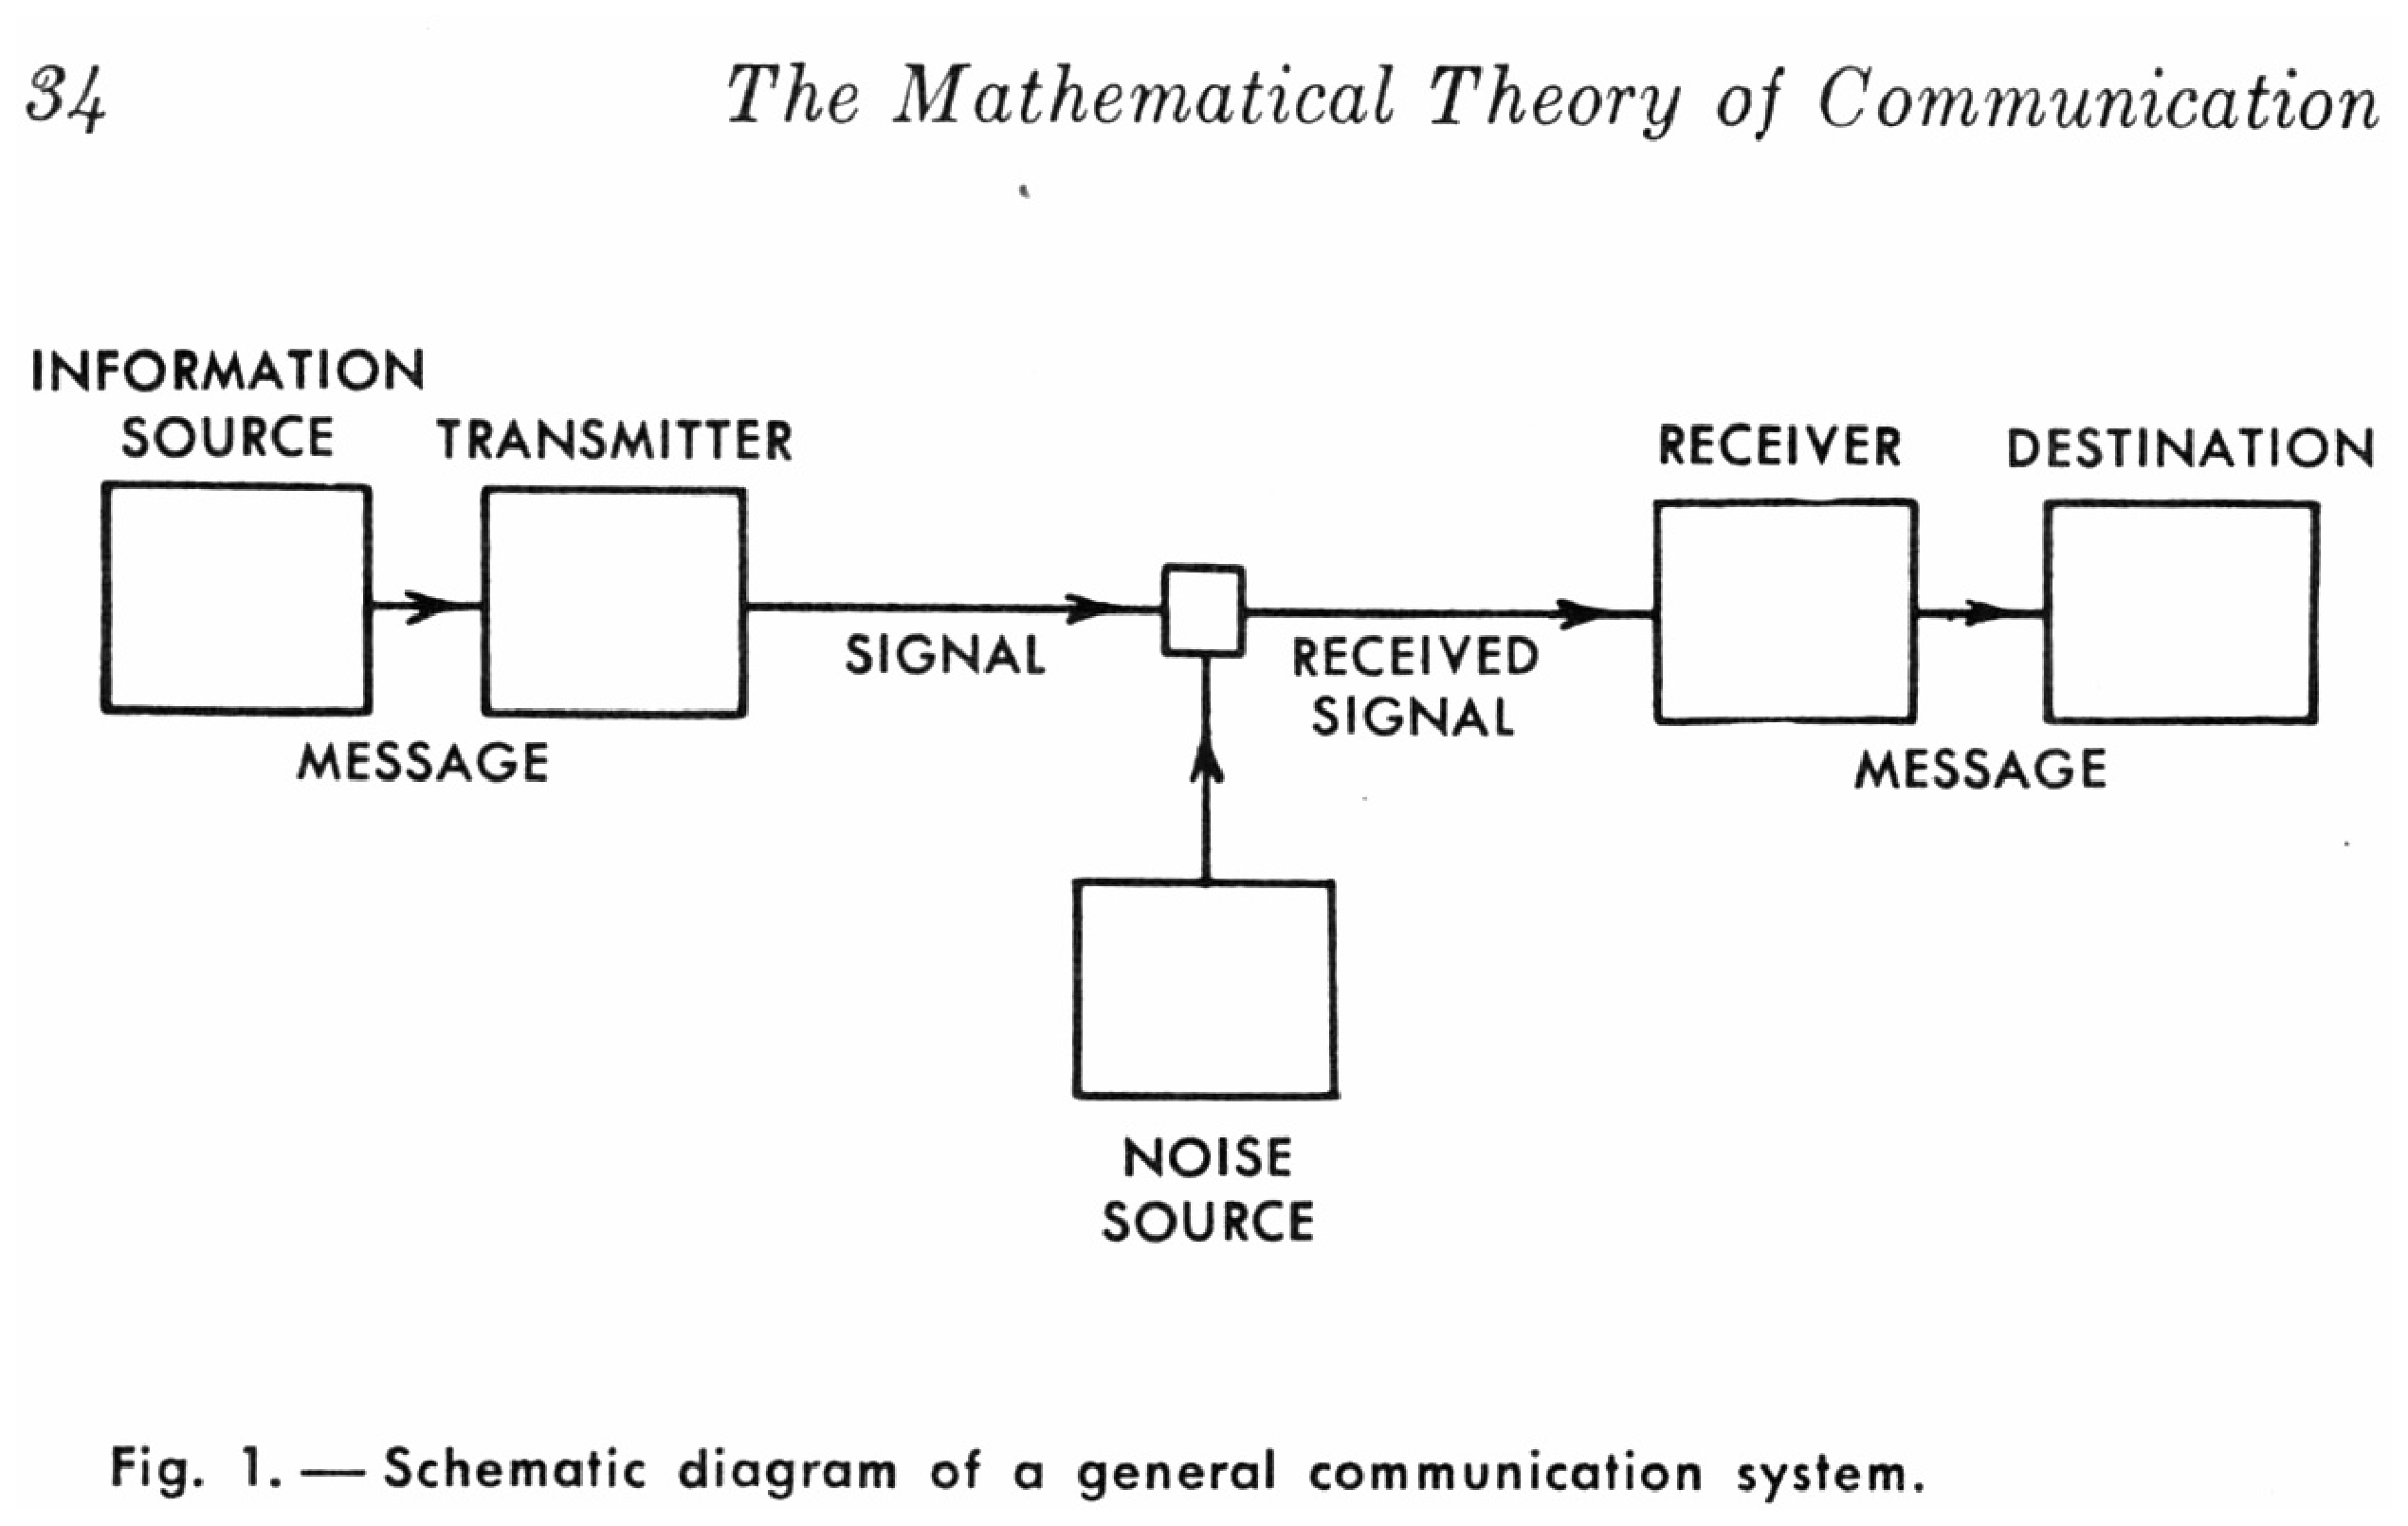
\includegraphics[height=0.9\textheight]{pics/shannon_comm_channel}
\end{center}


\myslide{Information as bits}
\MyLogo{Information Theory: $\log_2(x)$ is how many times you can
  divide $x$ by 2; if $y = \log_2(x)$ then $x = 2^y$} 
\begin{itemize}
\item Suppose we have 8 equally likely facts (A, B, C, \ldots H). 
 \\ How many yes-no  questions does it take to pinpoint one fact?\task

  \begin{itemize}
  \item This is the information in \txx{bits}
\\ you need $n$ bits of information
  \end{itemize}
  \item Technically the \txx{Entropy} \[ H(\mathrm{p}) = -\sum_{x \in X} \mathrm{p}(x)\log_2\mathrm{p}(x) \]
    \begin{itemize}
    \item We won't do all the maths
    \item Just think of things in terms of questions
    \end{itemize}
  \end{itemize}

\myslide{What if some facts are more common?}
\MyLogo{Information Theory}
\begin{itemize}
\item Simplified Polynesian (6 letters: p, k, i, u, t, a):
\\ Distribution:  p ($\frac{1}{8}$);
k ($\frac{1}{8}$);
i ($\frac{1}{8}$);
u ($\frac{1}{8}$);
   t ($\frac{1}{4}$);
   a ($\frac{1}{4}$)
\item We can do one letter in $2 \frac{1}{2}$ bits
  \begin{itemize}
  \item Is it (a or t) or (p, k, i, u), \ldots
  \end{itemize}
\item We can define a $2 \frac{1}{2}$ bit code 
  \begin{itemize}
  \item p (100); k (101); i (110); u (111); t (00);  a (01)  
  \end{itemize}
\item Which codes should be longer --- frequent or infrequent letters?
  \begin{itemize}
  \item What does this imply for language?
  \end{itemize}
\end{itemize}

%\citep[\S2.2]{Manning:Schuetze:1999}


\myslide{What if there is mutual information?}  
\MyLogo{Context Helps}
\begin{itemize}
\item \txx{Mutual information} measures the information that $X$ and $Y$ share:
how much does knowing one variable reduce our
uncertainty about the other.
\begin{itemize}
\item What is the next letter?
\item What is the next letter following \textit{t}?
\item What is the next letter following \textit{a}?
\item What is the next letter following \textit{q}?
\item What is the next letter following \textit{th}?
\item What is the next letter following \textit{as}?
\item What is the next letter following \textit{qu}?
\item What is the next letter following \textit{semanti}?
\end{itemize}
\item A language model and more context improves our guess
\end{itemize}


\myslide{Different Models for English}

Consider only 26 lowercase letters and a space, and a language model
based on probability (Hidden Markov Model).  How many guesses do we
need on average to guess the next letter?

\begin{itemize}
\item Zeroth order (random) = $\log_2$ 27 = 4.76
\item First order (frequency) = 4.03 \hfill (pick \textit{e})
\item Second order (one previous letter) = 2.8
\item Human (two previous letters) = 1.34
\end{itemize}

Surrounding context helps interpretation


\myslide{What if there is noise?}

\begin{itemize}
\item Imagine you want to send a signal, but randomly a bit gets flipped (noise)
  \begin{itemize}
  \item Original message /pa/ 100 01
  \item Received message /ka/ 101 01
  \end{itemize}
\item A very efficient model is weak to noise
\item If we make the message longer, we can guard against this
  \begin{itemize}
  \item Original message /pa/ 100 100 100 01 01 01
  \item Received message /ka/ 101 100 100 01 01 01
\\   We add \blu{redundancy} to the signal
\item There are much better encodings than this (\blu{Hamming codes})
\end{itemize}
\item Hmn lngge s vr rdndnt 
\end{itemize}

\myslide{Bandwidth}
\MyLogo{1 wpm $\approx$ 6x8 bits/60 seconds = 0.8 bits/second}
\begin{itemize}
\item \txx{Bandwidth} (or \txx{bit-rate}) is the maximum throughput of
  a logical or physical communication path in a digital communication
  system: e.g. how much information can be conveyed
\item Human Communication: words per minute (one word is 6 characters)
% 1 wpm = 6x8 bits/60 seconds = .8 bits/second 
\\ (English, computer science students, various studies)

\begin{tabular}{lrrl}
  Modality & Normal & Peak & Comment\\ \hline 
  Reading            & 300 & 200 &(proof reading is slower)\\
  Writing            & 31 & 21 &(composing) \\ 
  Speaking           & 150 & & (plus all kinds of tone/nuance)\\
  Hearing            & 150 & 210 &(speeded up)  \\
  Typing             & 33  & 19 &(composing) 
\end{tabular}
\item We adapt our communication depending on the bandwidth available

\end{itemize}

\myslide{Bandwidth of our Senses}
\MyLogo{\url{http://www.mu-sigma.com/uvnewsletter/index.html}}

\begin{center}
  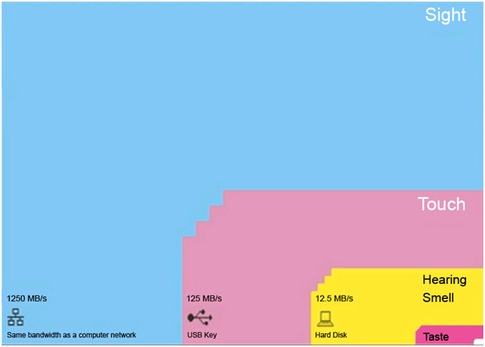
\includegraphics[height=0.95\textheight]{pics/bandwidth.png}  
\end{center}


% \myslide{The cloze test}
% \newcommand{\cz}[1]{\hspace*{3em}}

% Modern linguistics has been \cz{able} to provide theories and \cz{formalisms}
% for the specification of \cz{grammars} that express this mapping \cz{in} a
% declarative and transparent \cz{way}. Computational linguistics has
% contributed \cz{elaborate} platforms and tools for \cz{grammar} development.

% A few large \cz{scale} grammars have been \cz{designed} that exhibit sufficient
% \cz{accuracy} and coverage for \cz{real} application tasks. However,\cz{ these}
% encouraging developments were \cz{seriously} hampered by a \cz{lack} of methods
% for \cz{language} analysis that fulfill \cz{the} minimal requirements in
% \cz{efficiency}, robustness, and specificity.

% This simply \cz{means} that all \cz{systems} working with \cz{these} grammars have
% \cz{been} too slow \cz{and} too brittle \cz{for} real applications. \cz{Furthermore}, they
% have \cz{not} been able \cz{to} manage the \cz{vast} ambiguity in \cz{natural} language,
% i.e. \cz{they} could not \cz{select} among large \cz{numbers} of linguistically
% \cz{correct} analyses.

% \myslide{How did we go?}
% Modern linguistics has been {able} to provide theories and {formalisms}
% for the specification of {grammars} that express this mapping {in} a
% declarative and transparent {way}. Computational linguistics has
% contributed {elaborate} platforms and tools for {grammar} development.

% A few large scale grammars have been designed that exhibit sufficient
% accuracy and coverage for real application tasks. However, these
% encouraging developments were seriously hampered by a lack of methods
% for language analysis that fulfill the minimal requirements in
% efficiency, robustness, and specificity.

% This simply means that all systems working with these grammars have
% been too slow and too brittle for real applications. Furthermore, they
% have not been able to manage the vast ambiguity in natural language,
% i.e. they could not select among large numbers of linguistically
% correct analyses.

% \url{http://www.delph-in.net/index.php?page=1}


\myslide{Representing meaning}
\MyLogo{Also vector space, description, images, video, \ldots}
\begin{itemize}
\item One of our goals will be to represent meaning
\item There are various ways to do this
  \begin{itemize}
  \item Syntactic trees
  \item Logical forms
  \item Thesauri and Ontologies
  \item Translation
  \item Paraphrasing
  \end{itemize}
Can you think of others?

\item At the end of this course you should be able to use these to
  describe many aspects of meaning
\end{itemize}

\myslide{Language is normally under-specified}
\MyLogo{There are many meanings}
\begin{center}
\large We get \blu{words}: \\[2ex]
    \Large \eng{I saw a kid with a cat.} \\[3ex]
We want \emp{meaning}:
\\  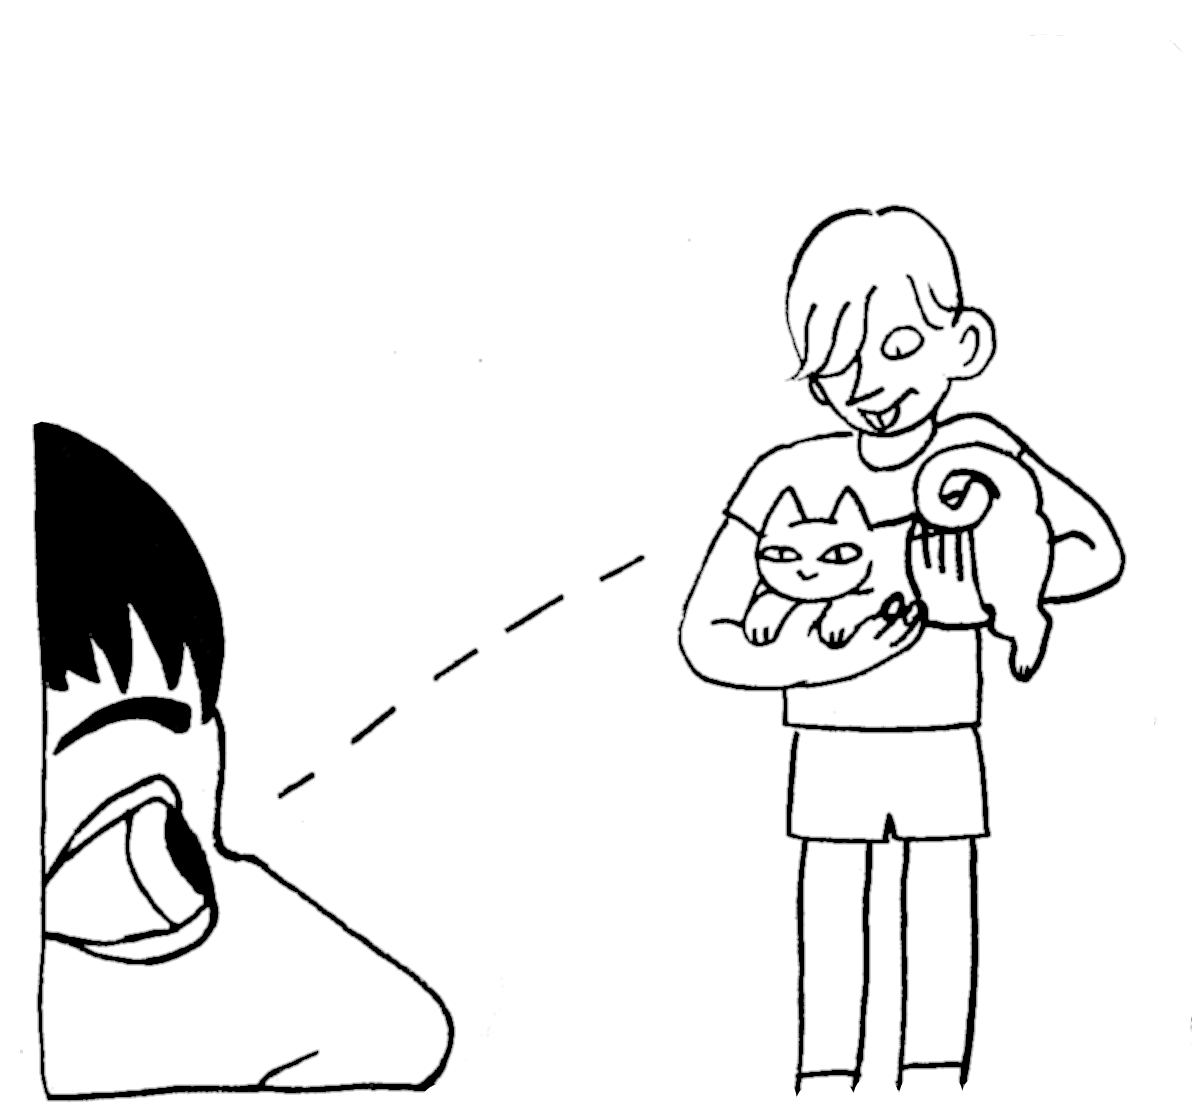
\includegraphics[width=0.3\textwidth]{pics/1.png}
\end{center}



\myslide{I saw a kid with a cat$_1$}
\MyLogo{Thanks to Eddy and Zina Pozen for the pictures}
\hspace{-3em}\begin{tabular}{ll}

  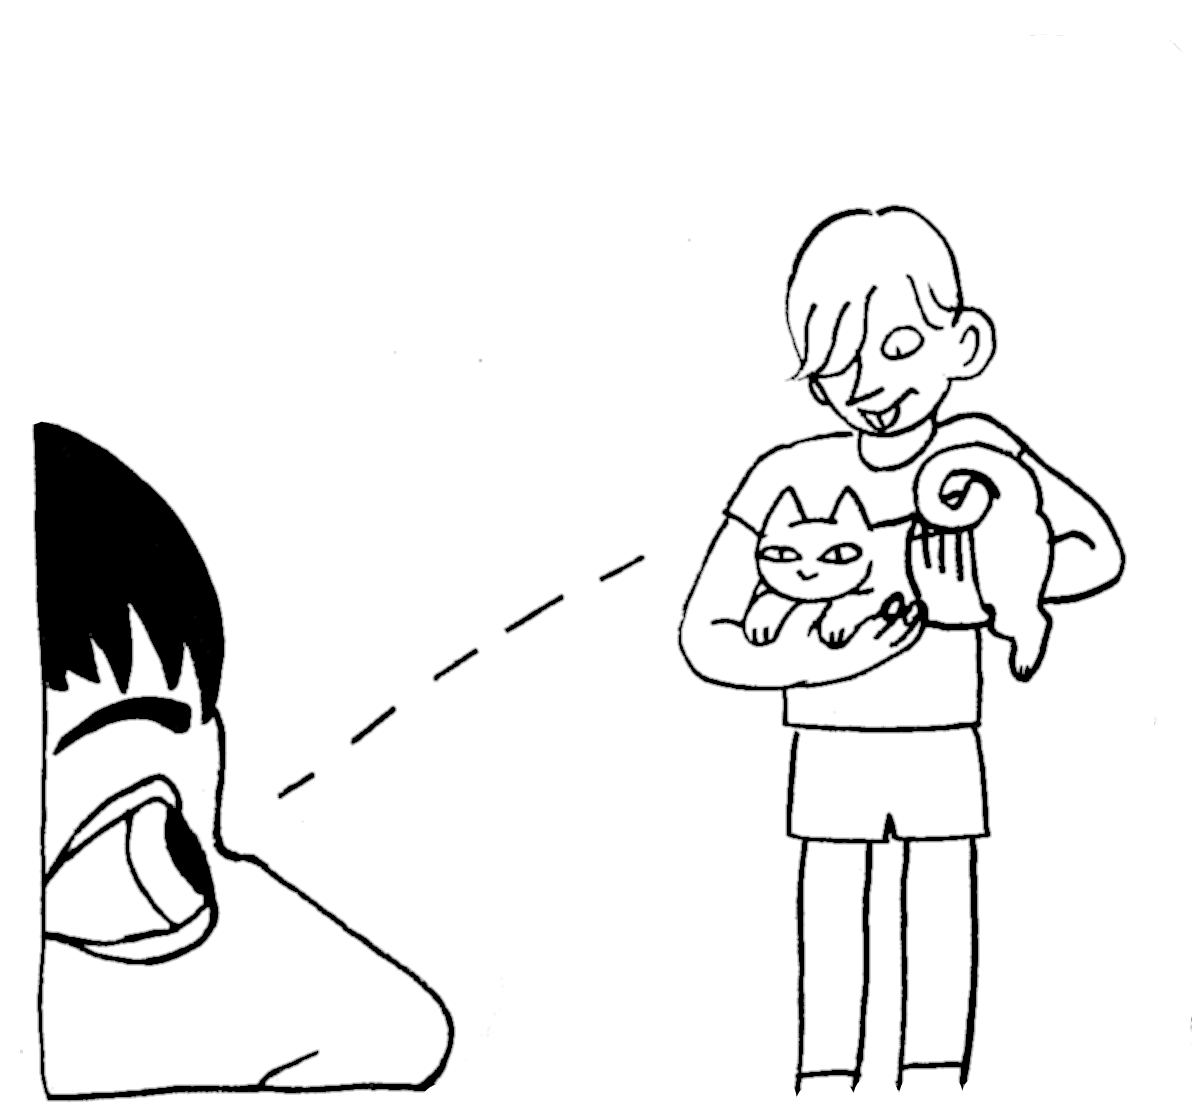
\includegraphics[width=0.5\textwidth]{pics/1.png}
&
  \begin{minipage}{0.45\textwidth}
    \vspace*{-10ex}
\begin{scriptsize}
 {%
 \leaf{\emph{I}}
 \branch{1}{NP}
 \leaf{\emph{saw}}
 \branch{1}{V:see}
 \leaf{\emph{a}}
 \branch{1}{DET}
 \leaf{\emph{kid}}
 \branch{1}{N}
 \leaf{\emph{with a cat}}
\branch{1}{PP[together]}
\branch{2}{\ibar{N}}
\branch{2}{NP}
 \branch{2}{VP}
 \branch{2}{S}
 \qobitree}
\end{scriptsize}
\\[5ex]
 \small \iz{see(I, kid: \textsc{past});  with(kid, cat)}
\\[1ex] \iz{see $\subset$ perceive}
\\ \iz{kid $\sim$ child}
\\ \iz{with $\subset$ together}
\end{minipage}

\end{tabular}

\myslide{I saw a kid with a cat$_2$}
\MyLogo{}
\hspace{-3em}\begin{tabular}{ll}
  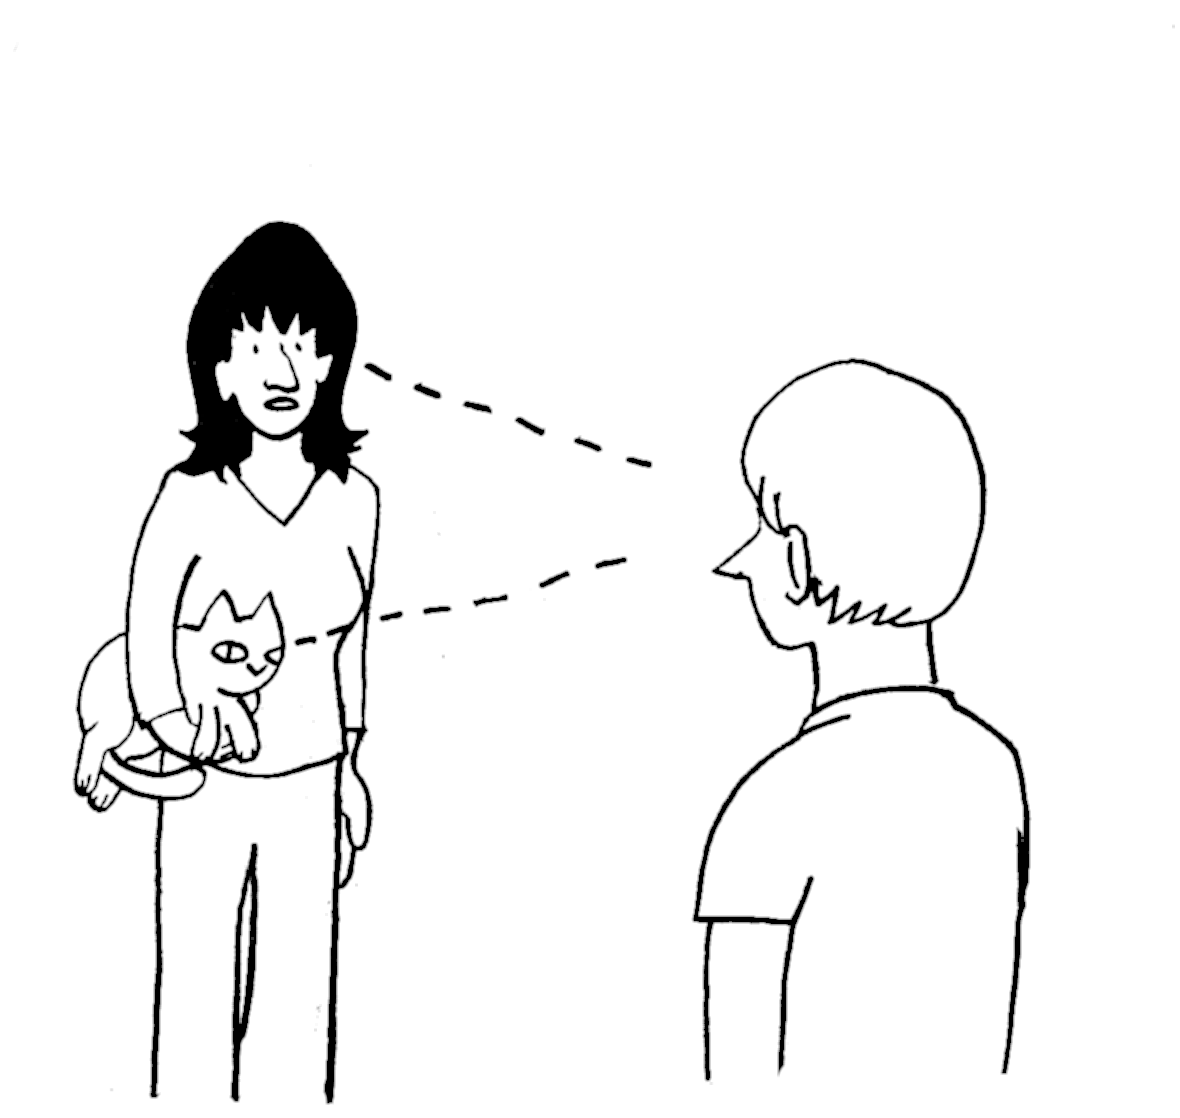
\includegraphics[width=0.5\textwidth]{pics/2.png}
&
  \begin{minipage}{0.45\textwidth}
    \vspace*{-15ex}
\begin{scriptsize}
 {%
 \leaf{\emph{I}}
 \branch{1}{NP}
 \leaf{\emph{saw}}
 \branch{1}{V:see}
 \leaf{\emph{a}}
 \branch{1}{DET}
 \leaf{\emph{kid}}
 \branch{1}{N}
\branch{2}{NP}
 \leaf{\emph{with a cat}}
\branch{1}{PP[together]}
 \branch{3}{VP}
 \branch{2}{S}
 \qobitree}
\end{scriptsize}
\\[3ex]
 \small 
 \iz{see(I, kid: \textsc{past}) with(I, cat)}
\\[1ex] \iz{see $\subset$ perceive}
\\ \iz{kid $\sim$ child}
\\ \iz{with $\subset$ together}
\end{minipage}
\end{tabular}




\myslide{I saw a kid with a cat$_3$}
\hspace{-3em}\begin{tabular}{ll}
  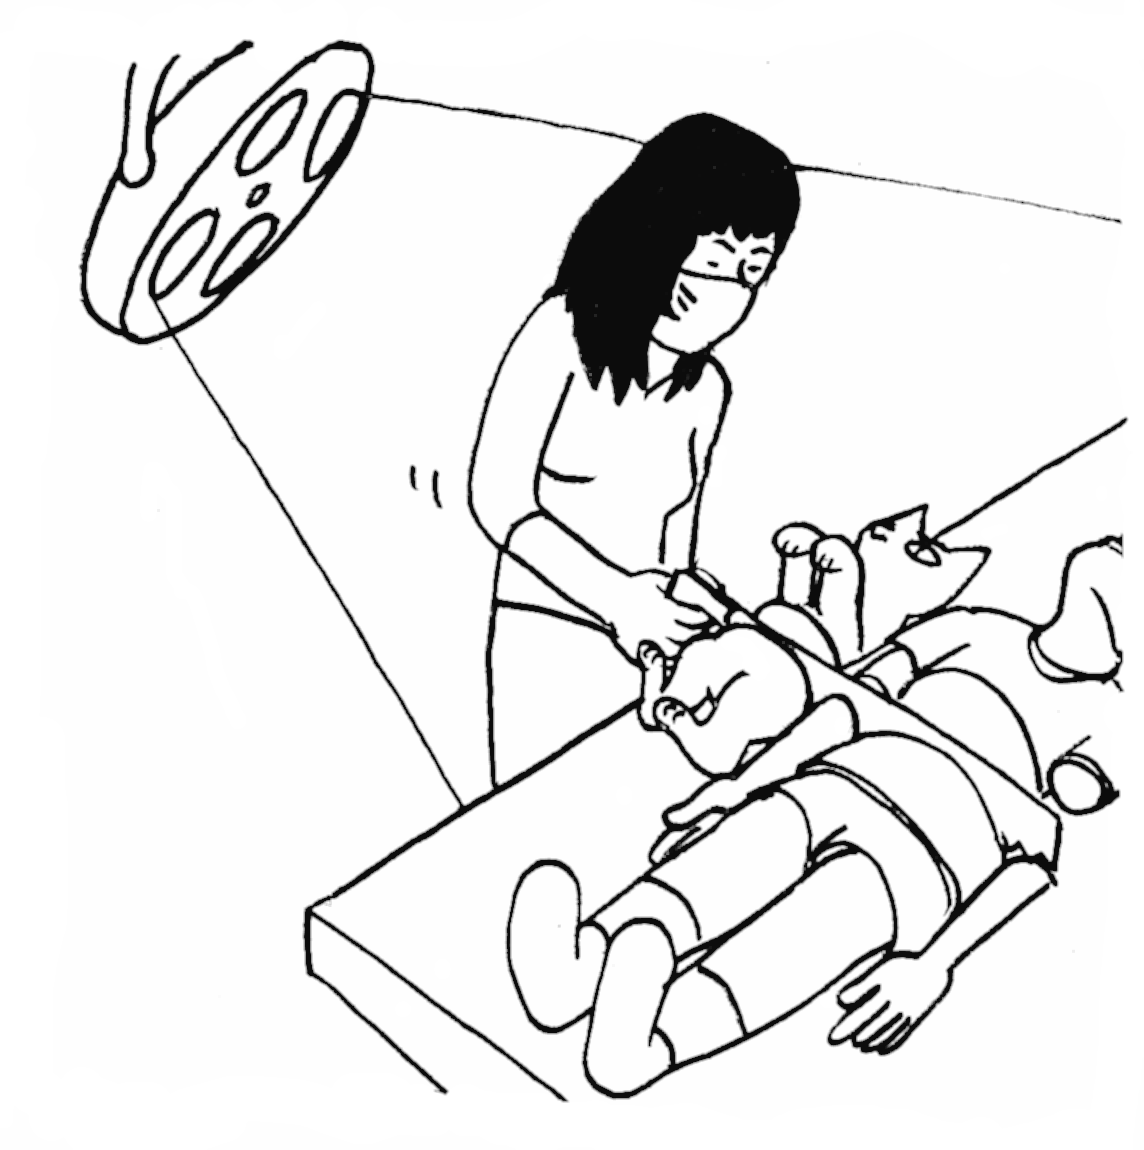
\includegraphics[width=0.5\textwidth]{pics/3.png}

&
  \begin{minipage}{0.45\textwidth}
    \vspace*{-15ex}
\begin{scriptsize}
 {%
 \leaf{\emph{I}}
 \branch{1}{NP}
 \leaf{\emph{saw}}
 \branch{1}{V:saw}
 \leaf{\emph{a}}
 \branch{1}{DET}
 \leaf{\emph{kid}}
 \branch{1}{N}
 \leaf{\emph{with a cat}}
\branch{1}{PP[together]}
\branch{2}{\ibar{N}}
\branch{2}{NP}
 \branch{2}{VP}
 \branch{2}{S}
 \qobitree}
\end{scriptsize}
\\[5ex]
 \small 
\iz{saw(I, kid: \textsc{pres});  with(kid, cat)}
\\[1ex] \iz{saw $\subset$ cut}
\\ \iz{kid $\sim$ child}
\\ \iz{with $\subset$ together}
\end{minipage}
\end{tabular}



\myslide{I saw a kid with a cat$_4$}
\hspace{-3em}\begin{tabular}{ll}
  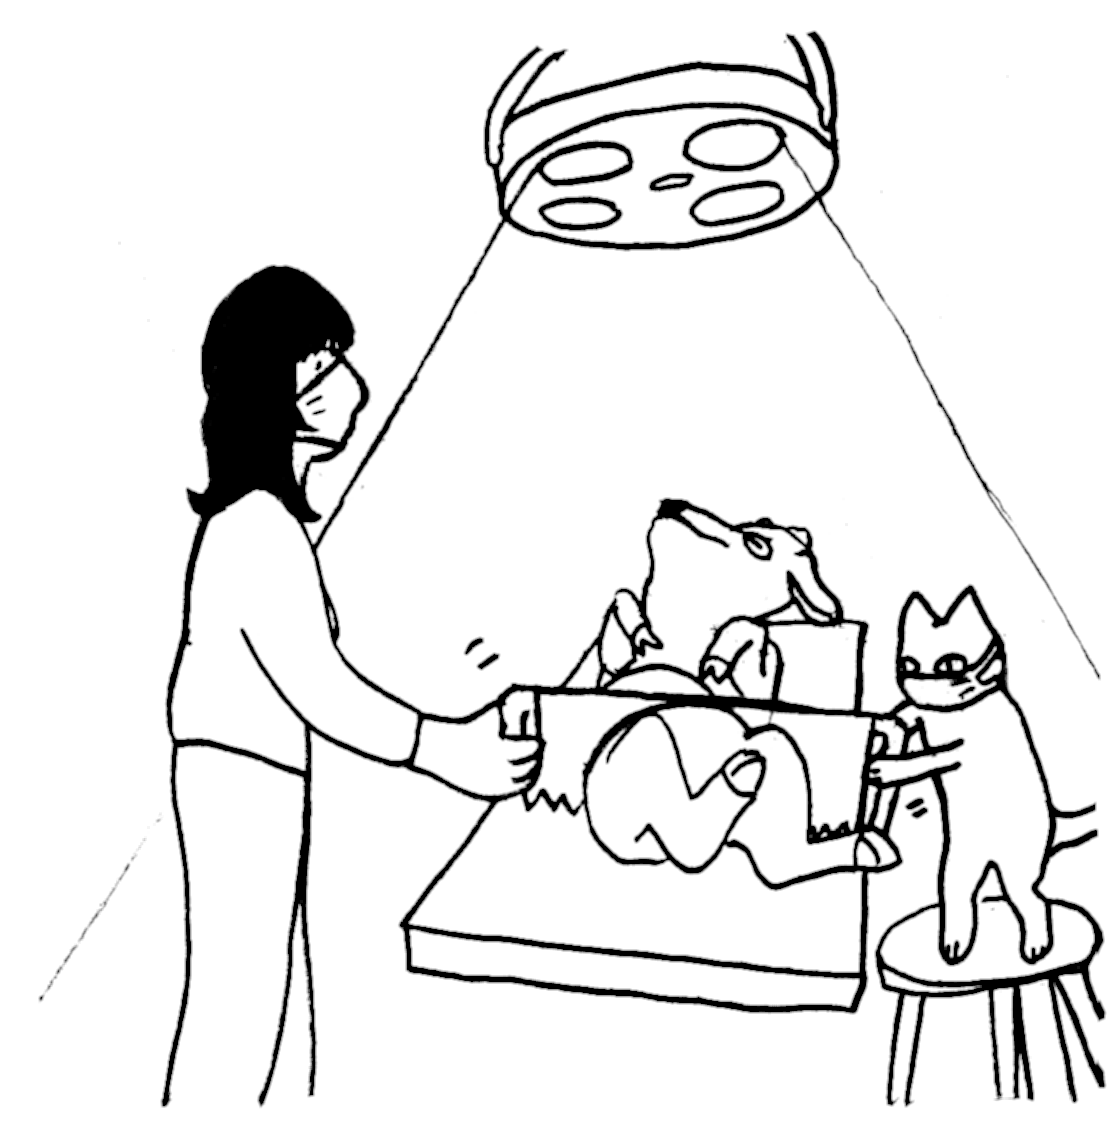
\includegraphics[width=0.5\textwidth]{pics/4.png}
&
  \begin{minipage}{0.45\textwidth}
    \vspace*{-15ex}
\begin{scriptsize}
 {%
 \leaf{\emph{I}}
 \branch{1}{NP}
 \leaf{\emph{saw}}
 \branch{1}{V:saw}
 \leaf{\emph{a}}
 \branch{1}{DET}
 \leaf{\makebox[1em]{\emph{kid} [goat]}}
 \branch{1}{N}
\branch{2}{NP}
 \leaf{\emph{with a cat}}
\branch{1}{PP[together]}
 \branch{3}{VP}
 \branch{2}{S}
 \qobitree}
\end{scriptsize}
\\[3ex]
 \small 
\iz{saw(I, kid: \textsc{present}) with(I, cat)}
\\[1ex] \iz{saw $\subset$ cut}
\\ \iz{kid $\sim$ young goat}
\\ \iz{with $\subset$ together}
\end{minipage}
\end{tabular}


\myslide{I saw a kid with a cat$_5$}
\hspace{-3em}\begin{tabular}{ll}
  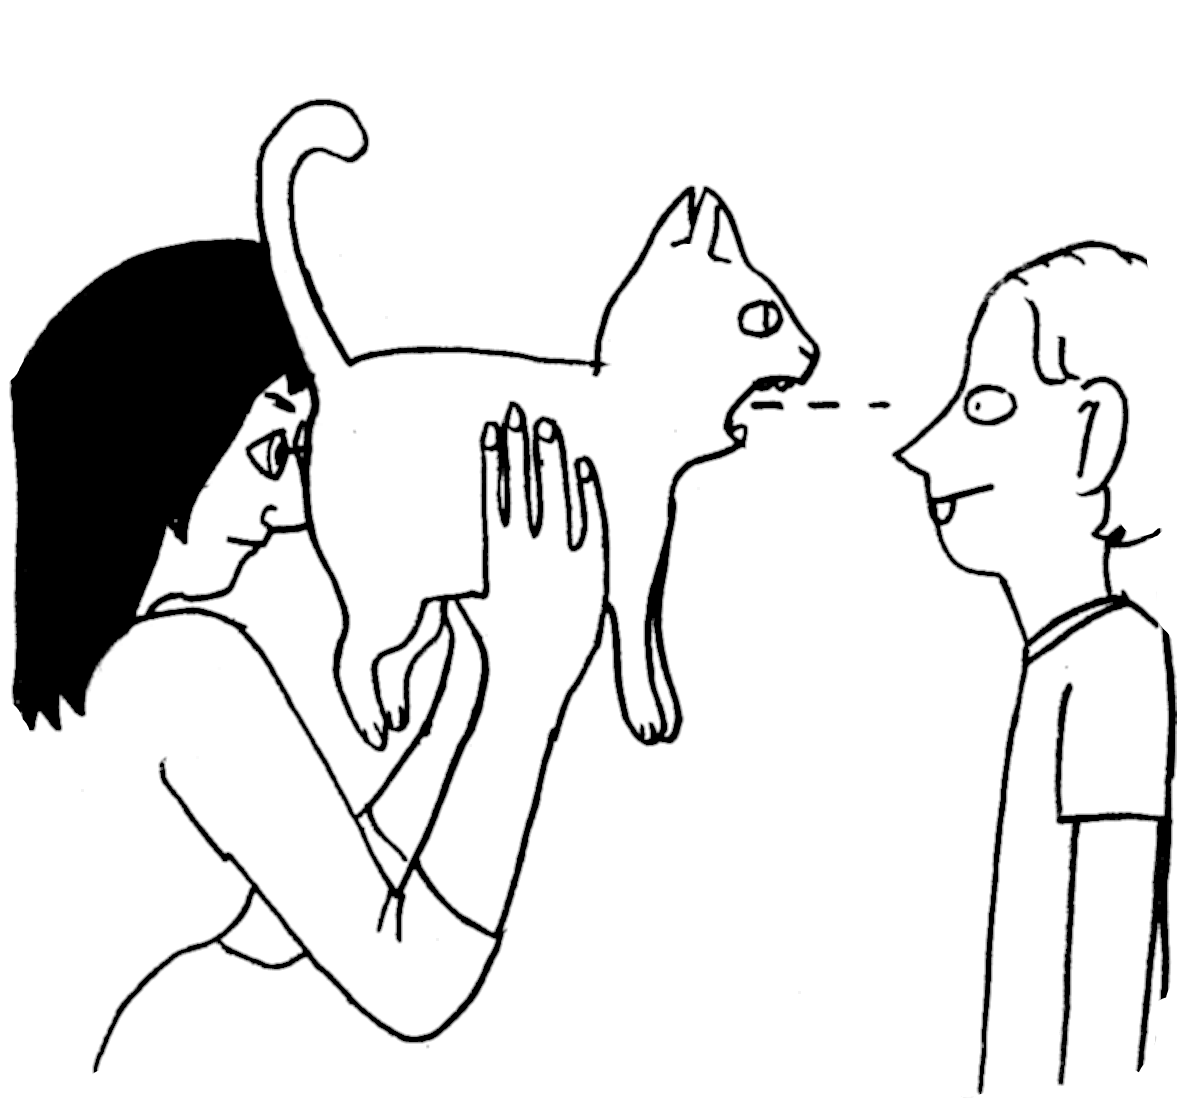
\includegraphics[width=0.5\textwidth]{pics/5.png}
&
  \begin{minipage}{0.45\textwidth}
    \vspace*{-15ex}
\begin{scriptsize}
 {%
 \leaf{\emph{I}}
 \branch{1}{NP}
 \leaf{\emph{saw}}
 \branch{1}{V:see}
 \leaf{\emph{a}}
 \branch{1}{DET}
 \leaf{\emph{kid}}
 \branch{1}{N}
\branch{2}{NP}
 \leaf{\emph{with a cat}}
\branch{1}{PP[instrument]}
 \branch{3}{VP}
 \branch{2}{S}
 \qobitree}
\end{scriptsize}
\\[3ex]
 \small 
 \iz{see(I, kid: \textsc{past}) with(I, cat) }
\\[1ex] \iz{see $\subset$ perceive}
\\ \iz{kid $\sim$ child}
\\ \iz{with $\subset$ instrumental}
 \end{minipage}
\end{tabular}


% \myslide{People are good at understanding}
% \MyLogo{We do this too}
% \begin{itemize}
% \item The words only hint at the meaning
% \item Many words can mean more than one thing (\blu{ambiguity})
% \item How can we \blu{model} and \blu{resolve} ambiguity?
% \item Look at the text and try to annotate the meaning
%   \begin{center}
%     Very hard work
%   \end{center}
% %   \begin{itemize}
% %   \item Deduce implicit models
% %     \begin{itemize}
% %     \item bag of words, $n$-gram chunks, \ldots
% %     \end{itemize}
% %   \item Define explicit models
% %     \begin{itemize}
% %     \item Grammars, lexicons and thesauri
% %     \end{itemize}
% %   \end{itemize}
% %\item Then build statistical language models (machine learning)
% \end{itemize}

\myslide{We can also use translations}
\makexeCJKactive
\begin{exe}
  \ex \glll 我 看到了 一个 抱着 猫 的 孩子 \\
  wǒ   kàndàole    yīgè   bàozhe  māo  de    háizi. \\
  I saw one holding cat 's child \\
  \trans I did see a child holding a cat

  \ex \glll 我 抱着 猫 看到了 一个 孩子 \\
  wǒ  bàozhe māo kàndàole  yīgè     háizi \\
  I holding cat saw one  child \\
 \trans I holding a cat did see a child

  \ex \glll 我 鋸锯  一个 孩子 和 他/她 的 猫 \\
wǒ jù  yīgè    háizi  hé  tā/tā   de māo \\
%wo3 ju4  yi1ge4    háizi  he2  ta1ta1   de ma1o\\
 I      saw    one    child   and     he/she  's cat\\
 \trans I saw  a child and their cat 

  \ex \glll 我 和 一只 猫 鋸锯 一只 小 山羊 \\
wǒ hē  yīzhǐ  māo jù yīzhǐ xiǎo  shānyáng  \\
%wo3 he1  yi1zhi3  ma1o ju4 yi1zhi3 xia3o  sha1nya2ng    \\
I and one cat saw one small goat \\

\trans I and a child saw a young goat
  \ex \glll 我 用 一只 猫 看到了 一个 孩子 \\
wǒ yòng yīzhǐ  māo kàndàole  yīgè  háizi \\
I use one cat saw one child \\
\trans Using a cat, I did see a child
\end{exe}
\makexeCJKinactive

\bigskip
\begin{center} \large
  Your turn: try to paraphrase --- translate into English
  \\ aim to be unambiguous, even if slightly disfluent
\end{center}

\myslide{Summary}
\MyLogo{Almost done}
\begin{itemize}
\item Syllabus; Administrivia
\item What is semantics?
\item Why should we be interested in semantics?
\item What is meaning?
\item Meaning as an open ended conceptual system
\item Semantic problems and solutions?
\item Information Theory (new!)
\end{itemize}

\emp{Next Week} Chapter 2: Meaning, Thought and Reality

\myslide{Acknowledgments and References}
\MyLogo{If I have seen further, it is by standing on the shoulders of giants (Isaac Newton)}
\begin{itemize}
\item Course design and slides inherit from Nala Lee's HG202 course,
  back in the depths of time (2009).
\item Thanks to Na-Rae Han for 
  inspiration for the student policies (from  \textit{LING 2050 Special Topics in Linguistics: Corpus linguistics}, U Penn; adapted).
  \item Further Reading: 
  \begin{itemize}
  \item  Shannon, C.E. (1948), "A Mathematical Theory of Communication", Bell System Technical Journal, 27, pp. 379–423 \& 623–656, July \& October, 1948. \url{http://cm.bell-labs.com/cm/ms/what/shannonday/shannon1948.pdf}
  \end{itemize}
\end{itemize}

\myslide{Bibliography}
% Reading: Jurafsky and Martin (2008) Chapter 20
\renewcommand{\section}[2]{}
\renewcommand{\baselinestretch}{0.9}
%\small
\bibliographystyle{aclnat}
\bibliography{abb,mtg,nlp,ling}



\end{document}



%%% Local Variables: 
%%% coding: utf-8
%%% mode: latex
%%% TeX-PDF-mode: t
%%% TeX-engine: xetex
%%% End: 

